\documentclass[11pt,letterpaper]{article}

\usepackage[utf8]{inputenc}
\usepackage[T1]{fontenc}
\usepackage[spanish,es-nodecimaldot,es-noshorthands,es-tabla,es-nolists]{babel}
\usepackage{mathptmx}
\usepackage[margin=2.5cm]{geometry}
\usepackage{amsmath,amssymb}
\usepackage{graphicx}
\usepackage{booktabs}
\usepackage{array}
\usepackage{url}
\usepackage[font=small,labelfont=bf]{caption}
\usepackage{enumitem}
\usepackage{microtype}
\usepackage{placeins}
\usepackage{tikz}
\usepackage{pgfplots}
\pgfplotsset{compat=1.17}
\usetikzlibrary{arrows.meta,positioning,fit,backgrounds}
\usepackage[hidelinks]{hyperref}

\setlength{\parskip}{0.2em}
\setlist{itemsep=0.2em,topsep=0.3em}

\begin{document}

% ------------------------------------------------------------------ Título
\begin{center}
{\LARGE\bfseries Detección de objetos 3D en nubes de puntos LiDAR\\[0.2em]
con convolución dispersa: entrenamiento y evaluación de SECOND en KITTI\par}
\vspace{1.2em}
{\large Juan Pablo Isaziga Benavides\par}
\vspace{0.3em}
Código 30000122025 \\
Programa de Ingeniería de Sistemas \\
Universidad de San Buenaventura Cali \\
Electiva de Ingeniería de Software --- Docente: Carlos Mario Paredes \\[0.4em]
Informe final del proyecto --- Noviembre de 2026
\end{center}

\vspace{0.5em}

% ---------------------------------------------------------------- Resumen
\begin{abstract}
\noindent Este trabajo entrena y evalúa un detector de objetos tridimensionales en nubes de puntos LiDAR. Tras revisar el estado del arte, organizado en torno a la representación por vóxeles y la convolución dispersa, se adopta SECOND, un detector de una etapa basado en convolución dispersa submanifold, y se especifica por completo su configuración. El modelo se entrenó desde cero durante 80 épocas sobre las 3\,712 escenas de entrenamiento de KITTI, en una tarjeta NVIDIA GeForce RTX 5060, y se evaluó sobre las 3\,769 escenas de validación con la precisión promedio oficial de 40 umbrales. Obtuvo una AP$_{3D}$ moderada de 81,09 en automóvil, 51,23 en peatón y 65,93 en ciclista, a menos de un punto de los pesos de referencia de OpenPCDet evaluados en las mismas condiciones y por encima del artículo original en automóvil. Un análisis de exhaustividad por distancia muestra que el desempeño se degrada con la lejanía: la exhaustividad de automóvil baja de 93,98\% en los primeros 20\,m a 55,59\% más allá de 40\,m, y la de peatón cae a 12,50\% en esa franja, en correspondencia con la escasez de puntos LiDAR que revela el análisis exploratorio. Los ejemplos cualitativos confirman que los errores se concentran en objetos lejanos y ocluidos.

\vspace{0.5em}
\noindent\textbf{Palabras clave:} nube de puntos, LiDAR, detección de objetos 3D, convolución dispersa, SECOND, KITTI.
\end{abstract}

% ============================================================ Introducción
\section{Introducción}

La detección de objetos tridimensionales a partir de nubes de puntos LiDAR es una de las tareas de percepción de las que depende un vehículo autónomo: el sistema de planificación necesita conocer la posición, el tamaño y la orientación de los automóviles, peatones y ciclistas que lo rodean \cite{qian2022, cai2025}. Formalmente, dada una nube de puntos $P = \{p_i\}_{i=1}^{N}$ con $p_i = (x_i, y_i, z_i, r_i)$, donde $r_i$ es la reflectancia, se busca predecir el conjunto de cajas delimitadoras orientadas $\{(x, y, z, l, w, h, \theta, c)\}$ de los objetos presentes en la escena, donde $c$ es la clase semántica \cite{geiger2013}. El desorden, la irregularidad y la dispersión de la nube impiden aplicar convoluciones densas de manera eficiente \cite{guo2021, li2021}, y sobre esa dificultad se construye la decisión de diseño central de este trabajo.

El objetivo del proyecto es entrenar un detector de aprendizaje profundo para esta tarea, evaluarlo con las métricas oficiales del \textit{benchmark} KITTI \cite{geiger2013} y comparar sus resultados con los publicados en la literatura. Se eligió SECOND \cite{yan2018}, un detector de una etapa basado en convolución dispersa, por ser la línea base más reproducible de su familia. El modelo se entrenó desde cero en el equipo del proyecto y se evaluó sobre el conjunto de validación; además se evaluaron los pesos preentrenados que publica la implementación de referencia, para separar el efecto del entrenamiento propio del de la arquitectura.

El documento se organiza así. La sección \ref{sec:estado} revisa el estado del arte y posiciona la propuesta. La sección \ref{sec:metodologia} describe el conjunto de datos, el preprocesamiento, la arquitectura y los protocolos de entrenamiento y evaluación. La sección \ref{sec:resultados} presenta los resultados, la sección \ref{sec:discusion} los interpreta y la sección \ref{sec:conclusiones} cierra con las conclusiones y el trabajo futuro. El código, el notebook con los resultados y los registros de ejecución están disponibles en \url{REPOSITORIO_PENDIENTE}.

% ========================================================== Estado del arte
\section{Estado del arte}
\label{sec:estado}

El primer avance clasificó los detectores según la forma en que consumen la nube de puntos, siguiendo el criterio de las revisiones sistemáticas disponibles \cite{qian2022, zamanakos2021, cai2025}. Esta sección retoma esa clasificación, profundiza en la familia que se adopta ---la basada en vóxeles con convolución dispersa--- y revisa las líneas de trabajo que compiten con ella o la extienden.

\subsection{Métodos basados en proyección}
\label{sec:proyeccion}

La primera estrategia para procesar nubes de puntos con redes convolucionales consistió en proyectarlas sobre un plano, generalmente la vista de pájaro o una imagen de rango, y aplicar después una red 2D convencional \cite{qian2022, zamanakos2021}. PIXOR \cite{yang2018} es el ejemplo representativo: discretiza la vista de pájaro en una rejilla de ocupación y altura y predice las cajas en tiempo real con una red de una etapa. Estos métodos son rápidos porque operan sobre tensores densos y regulares, pero la proyección descarta parte de la información geométrica y hace que objetos cercanos entre sí colapsen en la misma región del mapa \cite{cai2025}.

\subsection{Representación por vóxeles y convolución dispersa}
\label{sec:voxeles}

VoxelNet \cite{zhou2018} fue el primer detector entrenable de extremo a extremo sobre vóxeles. Divide el espacio en una rejilla tridimensional, codifica los puntos de cada celda ocupada mediante una capa de codificación de atributos de vóxel y aplica convoluciones 3D densas. Su limitación es estructural: al operar sobre un tensor denso, la red gasta la mayor parte del cómputo en celdas vacías, que en una escena LiDAR típica son la gran mayoría del volumen \cite{zamanakos2021}.

SECOND \cite{yan2018} resolvió ese cuello de botella sustituyendo las convoluciones 3D densas por convoluciones dispersas submanifold. Estas solo evalúan el núcleo en las posiciones ocupadas y preservan el patrón de dispersión entre capas. Los autores reportan una aceleración de cuatro veces en entrenamiento y de tres en inferencia frente a la red densa equivalente, con exactitud competitiva. La convolución dispersa pasó de ser una optimización a convertirse en el componente estándar de los detectores posteriores \cite{ke2025, ao2026}.

PointPillars \cite{lang2019} tomó un camino intermedio entre la proyección y los vóxeles: agrupa los puntos en columnas verticales, lo que elimina por completo la convolución 3D y permite construir un mapa pseudoimagen procesable con una red 2D. Gana velocidad a costa de resolución vertical, un compromiso desfavorable para objetos bajos. SP-Pillars \cite{chen2025sp} mantiene esa representación y añade una red de atributos de columna ponderada y una red de percepción multiescala, con el objetivo explícito de equilibrar exactitud y velocidad.

\subsection{Refinamientos sobre la línea base SECOND}

Como SECOND se consolidó como línea base, buena parte de la literatura reciente se formula como mejora sobre ella, lo que facilita la comparación cuantitativa.

Ke et al. \cite{ke2025} identifican que la codificación de un solo canal en la etapa de vóxel es insuficiente y proponen un módulo que fusiona atributos locales y globales combinando convolución con autoatención. Reportan un mAP de 69,08\% con codificación por vóxeles frente a 67,87\% con codificación por columnas, lo que respalda la representación volumétrica. FGVoxel3D \cite{ao2026} cuestiona el supuesto de resolución única: no existe un tamaño de vóxel óptimo para todas las clases, y por eso propone una extracción multirresolución que mejora en 3,52\% el mAP de automóvil de SECOND en el conjunto de prueba de KITTI. Esa cifra cuantifica el margen de mejora que queda sobre la configuración que este proyecto implementa.

HFSA-Net \cite{yin2026} actúa sobre los tres bloques del detector: un codificador estructurado de vóxeles, una red troncal con atención híbrida y una cabeza que agrega escalas para objetos de distinto tamaño. Con ello obtiene un aumento de 3,34\% de mAP sobre su línea base en KITTI. Focals Conv \cite{chen2022b} observa que tratar todos los vóxeles ocupados con igual importancia desperdicia capacidad, y propone una convolución dispersa focal que concentra el aprendizaje en los vóxeles relevantes. IAVT-SSD \cite{wang2025iavt} señala que los detectores de una etapa son vulnerables al ruido de fondo y lo aborda con un muestreo ponderado consciente de instancias que descarta los puntos de reflexión del suelo. Una vía distinta reintroduce conocimiento geométrico explícito, agrupando candidatos con criterios clásicos antes de alimentar la red aprendida \cite{shi2025}.

\subsection{Métodos basados en puntos y detectores de dos etapas}

PointRCNN \cite{shi2019} introdujo el esquema de dos etapas sobre puntos: una primera red genera propuestas a partir de los puntos segmentados como primer plano y una segunda las refina en coordenadas canónicas. Su extensión posterior incorporó información de partes del objeto para guiar el refinamiento \cite{shi2021}. PV-RCNN \cite{shi2020} combinó ambas representaciones, usando una red dispersa de vóxeles para generar propuestas y un conjunto de puntos clave para agregar contexto. Voxel R-CNN \cite{deng2021} mostró que el refinamiento puede hacerse directamente sobre atributos de vóxel, sin volver a los puntos, con exactitud comparable y menor costo.

La misma tensión entre exactitud y costo aparece en trabajos recientes. SPS-RCNN \cite{xu2025} es un detector punto-vóxel de varias etapas que usa un muestreo de propuestas guiado por semántica para aumentar la proporción de puntos de primer plano, y una atención en cascada orientada a objetos de rango medio y lejano.

\subsection{Detectores libres de anclas}

CenterPoint \cite{yin2021} reemplazó las anclas predefinidas por la predicción directa del centro del objeto en un mapa de calor, eliminando la necesidad de ajustar tamaños y umbrales de asignación por clase. El enfoque se impone en conjuntos de 360 grados con muchas clases, donde el diseño manual de anclas se vuelve impracticable, pero su ventaja es menor en KITTI, donde solo se evalúan tres clases de geometría bien definida.

\subsection{Objetos lejanos y clases minoritarias}

El desempeño en peatones, ciclistas y objetos distantes sigue siendo el punto débil compartido por todas las familias. Zhao et al. \cite{zhao2025} combinan un grafo que modela la geometría local con un árbol que captura el contexto jerárquico, y adaptan el intercambio de mensajes a la densidad de puntos. En el nivel moderado de KITTI superan a su referencia en 2,59\% para automóvil, 0,49\% para peatón y 3,05\% para ciclista. EAS-Det \cite{wang2025eas} propone un módulo acoplable que fusiona información de bordes con contexto semántico para preservar los contornos del objeto, y reporta ganancias de hasta 10,34\% de AP en peatones y 8,66\% en ciclistas sobre KITTI. La magnitud de estas ganancias, muy superior a la obtenida en automóviles, confirma que las clases minoritarias son donde existe más margen.

\subsection{Eficiencia computacional}

La percepción debe ejecutarse dentro del ciclo de control del vehículo, lo que convierte la latencia en una restricción de diseño y no en una métrica secundaria. Erabati y Araujo \cite{erabati2024b} proponen un transformador de vóxeles ligero orientado a reducir el costo del mecanismo de atención, y SP-Pillars \cite{chen2025sp} persigue el mismo objetivo desde la representación por columnas.

\subsection{Fusión multimodal y robustez}

La fusión de LiDAR y cámara busca aprovechar sensores complementarios, y existe un cuerpo consolidado de propuestas y revisiones al respecto \cite{erabati2024a, liu2023, pravallika2024}. Su costo es la dependencia de una calibración precisa entre sensores y un mayor consumo de cómputo \cite{qian2022}.

En cuanto a la robustez, Dong et al. \cite{dong2023} construyen un banco de pruebas de corrupciones comunes y muestran que el desempeño reportado en condiciones ideales no se transfiere a escenarios degradados. Li et al. \cite{li2026} abordan ese problema con un módulo de condicionamiento de la nube basado en vecinos más cercanos que se antepone a un detector sin modificarlo; lo evalúan precisamente sobre SECOND, PointPillars y Voxel R-CNN en KITTI, con mejoras consistentes bajo ruido y puntos atípicos. Para clima adverso, la literatura ha propuesto restricciones geométricas \cite{qi2024}, aumentación basada en instancias \cite{an2026}, destilación de conocimiento \cite{liu2025} y simulación física de nieve sobre nubes reales \cite{ju2026}.

\subsection{Análisis comparativo y posicionamiento de la propuesta}

La Tabla \ref{tab:comparativa} resume los trabajos revisados y su relación con la propuesta de este proyecto.

\begin{table}[htbp]
\caption{Análisis comparativo de los trabajos revisados frente a la propuesta.}
\label{tab:comparativa}
\centering
\footnotesize
\renewcommand{\arraystretch}{1.15}
\begin{tabular}{@{}>{\raggedright\arraybackslash}p{2.6cm}>{\raggedright\arraybackslash}p{2.1cm}>{\raggedright\arraybackslash}p{4.6cm}>{\raggedright\arraybackslash}p{6.1cm}@{}}
\toprule
\textbf{Trabajo} & \textbf{Representación} & \textbf{Aporte principal} & \textbf{Relación con la propuesta} \\
\midrule
PIXOR \cite{yang2018} & Proyección BEV & Detección en tiempo real sobre vista de pájaro & Descartado: pierde información geométrica \\
VoxelNet \cite{zhou2018} & Vóxeles densos & Primer detector de extremo a extremo sobre vóxeles & Antecedente directo; descartado por el costo de la convolución densa \\
SECOND \cite{yan2018} & Vóxeles dispersos & Convolución dispersa submanifold & \textbf{Arquitectura adoptada}; define la línea base a reproducir \\
PointPillars \cite{lang2019} & Columnas & Elimina la convolución 3D & Descartado por la pérdida de resolución vertical \\
SP-Pillars \cite{chen2025sp} & Columnas & Atributos ponderados y percepción multiescala & Referencia del compromiso exactitud--velocidad \\
PointRCNN \cite{shi2019} & Puntos & Propuestas desde segmentación de primer plano & Mayor exactitud, costo fuera del alcance \\
PV-RCNN \cite{shi2020} & Híbrida & Abstracción punto-vóxel con puntos clave & Posible extensión posterior \\
Voxel R-CNN \cite{deng2021} & Vóxeles dispersos & Refinamiento sobre atributos de vóxel & Ruta natural de mejora sobre la línea base \\
SPS-RCNN \cite{xu2025} & Híbrida & Muestreo de propuestas guiado por semántica & Muestra la ganancia de las dos etapas en rango lejano \\
CenterPoint \cite{yin2021} & Vóxeles / columnas & Predicción de centros sin anclas & Ventaja marginal con tres clases evaluadas \\
Focals Conv \cite{chen2022b} & Vóxeles dispersos & Convolución dispersa focal & Módulo sustituible dentro de la red troncal \\
Ke et al.\ \cite{ke2025} & Vóxeles dispersos & Fusión de atributos locales y globales & Evidencia a favor de vóxeles frente a columnas \\
FGVoxel3D \cite{ao2026} & Multirresolución & Vóxeles de resolución variable & Cuantifica el margen sobre SECOND (+3,52\%) \\
HFSA-Net \cite{yin2026} & Vóxeles dispersos & Codificación estructurada y atención híbrida & Mejora de +3,34\% de mAP en KITTI \\
IAVT-SSD \cite{wang2025iavt} & Vóxeles dispersos & Muestreo consciente de instancias & Mitiga el ruido del suelo que afecta a la propuesta \\
Zhao et al.\ \cite{zhao2025} & Grafo y árbol & Paso de mensajes adaptado a la densidad & Ataca la degradación en objetos lejanos \\
EAS-Det \cite{wang2025eas} & Acoplable & Fusión de bordes y semántica & Mayor ganancia en peatón y ciclista \\
Li et al.\ \cite{li2026} & Preprocesamiento & Condicionamiento de la nube degradada & Evaluado sobre SECOND; extensión de robustez \\
Dong et al.\ \cite{dong2023} & --- & Banco de corrupciones comunes & Justifica declarar la limitación climática de KITTI \\
\bottomrule
\end{tabular}
\end{table}

De la tabla se desprende la decisión de diseño. La familia de vóxeles dispersos concentra la línea base más reproducible y la mayoría de las extensiones recientes, de modo que cualquier resultado obtenido sobre ella es directamente comparable con la literatura. Los métodos de dos etapas y los multimodales ofrecen mayor exactitud, pero su costo de entrenamiento y su dependencia de calibración los sitúan fuera del alcance de este proyecto. Por tanto se adopta SECOND, con el objetivo de entrenarlo, reproducir su desempeño publicado e identificar dónde falla, como punto de partida para incorporar después uno de los módulos de mejora identificados.

% ================================================================ Metodología
\section{Metodología}
\label{sec:metodologia}

\subsection{Conjunto de datos}

Se utiliza el \textit{KITTI 3D Object Detection Benchmark} \cite{geiger2013}, publicado por el Karlsruhe Institute of Technology y el Toyota Technological Institute at Chicago y disponible en \url{https://www.cvlibs.net/datasets/kitti/}. La Tabla \ref{tab:dataset} consolida sus características.

\begin{table}[htbp]
\caption{Características del conjunto de datos KITTI.}
\label{tab:dataset}
\centering
\small
\renewcommand{\arraystretch}{1.15}
\begin{tabular}{@{}>{\raggedright\arraybackslash}p{4cm}>{\raggedright\arraybackslash}p{11cm}@{}}
\toprule
\textbf{Atributo} & \textbf{Valor} \\
\midrule
Muestras & 7\,481 de entrenamiento (con etiquetas) y 7\,518 de prueba (sin etiquetas públicas) \\
Objetos anotados & 80\,256 \\
Clases anotadas & 8: \textit{Car}, \textit{Van}, \textit{Truck}, \textit{Pedestrian}, \textit{Person\_sitting}, \textit{Cyclist}, \textit{Tram}, \textit{Misc} \\
Clases evaluadas & 3: automóvil, peatón y ciclista \\
Sensor LiDAR & Velodyne HDL-64E: 64 haces, 10\,Hz, resolución angular de 0,09\textdegree, precisión de 2\,cm, alcance de 120\,m, del orden de $10^5$ puntos por barrido \\
Resolución de imagen & Aproximadamente $1242 \times 375$ píxeles (varía ligeramente entre secuencias) \\
Campo anotado & Frontal, de aproximadamente 90\textdegree{} y hasta unos 70\,m \\
Tamaño en disco & 29\,GB de nubes de puntos, 12\,GB de imágenes, 16\,MB de calibración y 5\,MB de etiquetas \\
Condiciones de captura & Diurnas y con clima favorable, en zonas urbanas, rurales y autopistas de Karlsruhe \\
Licencia & Creative Commons Atribución-NoComercial-CompartirIgual 3.0 \\
\bottomrule
\end{tabular}
\end{table}

La licencia permite el uso académico con atribución, prohíbe el uso comercial y obliga a compartir las obras derivadas bajo los mismos términos. Este proyecto cumple esas condiciones por ser un trabajo de curso sin fines comerciales.

Cada muestra se compone de cuatro archivos: la nube de puntos en formato binario, con $N \times 4$ valores de coma flotante $(x, y, z, r)$; la imagen de la cámara color izquierda; las matrices de calibración entre LiDAR y cámara, y un archivo de etiquetas con una línea por objeto. Cada línea de etiqueta contiene la clase (categórica), el truncamiento (continua en $[0,1]$), la oclusión (entera de 0 a 3), el ángulo de observación, la caja 2D en la imagen, las dimensiones alto, ancho y largo en metros, la posición del centro en metros y la rotación $\theta$ alrededor del eje vertical.

La distribución de clases está marcadamente desbalanceada. Según el conteo propio sobre las etiquetas de entrenamiento (sección \ref{sec:resultados}), el automóvil reúne el 70,8\% de los objetos anotados, el peatón el 11,1\%, la furgoneta el 7,2\%, el ciclista el 4,0\%, el camión el 2,7\%, la categoría miscelánea el 2,4\%, el tranvía el 1,3\% y la persona sentada el 0,5\%, proporciones que coinciden con las reportadas en \cite{wirges2018}. Este desbalance condiciona la estrategia de aumentación y explica por qué las métricas de peatón y ciclista quedan por debajo de las de automóvil en toda la literatura revisada.

\subsection{Justificación del conjunto}

La elección se sostiene en cuatro argumentos. El primero es la correspondencia: el conjunto fue construido para esta tarea exacta, de modo que no requiere reetiquetado ni adaptación. El segundo es la comparabilidad cuantitativa: casi todos los trabajos de la Tabla \ref{tab:comparativa} reportan sobre KITTI bajo el mismo protocolo oficial, lo que permite situar los resultados propios frente a cifras publicadas. El tercero es la viabilidad: con 7\,481 muestras anotadas y 29\,GB de nubes de puntos, el conjunto es manejable en una sola tarjeta gráfica, a diferencia de nuScenes \cite{caesar2020}, que supera los 390\,000 barridos. El cuarto es la pertinencia frente al vacío identificado: la estratificación oficial en niveles de dificultad permite medir directamente la degradación en objetos ocluidos y lejanos.

Las limitaciones se declaran de forma explícita. KITTI no contiene escenas nocturnas ni de clima adverso, por lo que no permite abordar la robustez climática. Sus anotaciones cubren solo el campo frontal. Su tamaño reducido incrementa el riesgo de sobreajuste, lo que vuelve obligatoria la aumentación de datos. Además, un modelo ajustado a un único sensor y una única ciudad no se transfiere directamente a otros dominios \cite{sohail2025}, de modo que las cifras obtenidas deben leerse como específicas de este conjunto.

\subsection{Partición de los datos}

Como las etiquetas del conjunto de prueba no son públicas, se adopta la partición propuesta por Chen et al. \cite{chen2015} y usada desde entonces por la mayoría de la literatura \cite{yan2018, shi2020, deng2021}: 3\,712 muestras para entrenamiento y 3\,769 para validación. Ambos subconjuntos provienen de secuencias de video distintas, lo que evita que cuadros consecutivos de una misma secuencia aparezcan a la vez en entrenamiento y validación e inflen artificialmente las métricas.

\subsection{Preprocesamiento}

El preprocesamiento reproduce la configuración oficial de la arquitectura \cite{yan2018} en la implementación de referencia \cite{openpcdet}, y consta de cuatro etapas.

\textbf{Recorte al campo de visión.} Se conservan solo los puntos que caen dentro del campo de visión de la cámara, porque fuera de él no hay anotaciones y esos puntos solo aportarían fondo sin etiqueta.

\textbf{Recorte del rango.} Se descartan los puntos fuera del volumen de interés, definido como $x \in [0;\, 70{,}4]$, $y \in [-40;\, 40]$ y $z \in [-3;\, 1]$ metros en el sistema de coordenadas del LiDAR. Durante el entrenamiento, además, el orden de los puntos se baraja aleatoriamente en cada iteración.

\textbf{Voxelización.} El volumen se discretiza con vóxeles de $0{,}05 \times 0{,}05 \times 0{,}1$\,m, lo que produce una rejilla de $1408 \times 1600 \times 40$ celdas en $(x, y, z)$. Se retienen como máximo $T = 5$ puntos por vóxel y 16\,000 vóxeles no vacíos por escena en entrenamiento, ampliados a 40\,000 en inferencia.

\textbf{Codificación de atributos.} Cada vóxel ocupado se representa por la media de los atributos de sus puntos, $(\bar{x}, \bar{y}, \bar{z}, \bar{r})$. Se opta por esta codificación simple en lugar de la red de codificación aprendida de VoxelNet \cite{zhou2018} porque, con vóxeles de este tamaño, la variabilidad dentro de cada vóxel es baja y el costo adicional no se justifica.

\subsection{Aumentación de datos}

Dado el tamaño reducido del conjunto, se aplican las cuatro transformaciones propuestas en \cite{yan2018}, cuya efectividad confirman trabajos posteriores sobre la misma línea base \cite{ke2025, ao2026}:

\begin{itemize}
\item \textbf{Muestreo de objetos reales.} Se construye previamente una base de datos con los puntos de cada objeto anotado, descartando los que tienen menos de cinco puntos. En cada iteración se insertan en la escena hasta 20 automóviles, 15 peatones y 15 ciclistas tomados de esa base, apoyados sobre el plano de la calzada de la escena (los planos estimados que distribuye la implementación de referencia \cite{openpcdet}) y sin superponerse a los objetos existentes. Esta técnica ataca directamente el desbalance de clases.
\item \textbf{Reflexión aleatoria} respecto al eje $x$.
\item \textbf{Rotación global} con un ángulo muestreado uniformemente en $[-\pi/4,\, \pi/4]$.
\item \textbf{Escalamiento global} con un factor en $[0{,}95;\, 1{,}05]$.
\end{itemize}

\subsection{Arquitectura propuesta}

Se implementa SECOND \cite{yan2018}, organizado en cuatro bloques encadenados: codificación de vóxeles, red troncal dispersa 3D, red troncal 2D en vista de pájaro y cabeza de detección basada en anclas. La Figura \ref{fig:arquitectura} presenta el esquema general y la Tabla \ref{tab:capas} detalla las capas tal como aparecen en la implementación de referencia \cite{openpcdet}.

\begin{figure}[htbp]
\centering
\resizebox{\textwidth}{!}{%
\begin{tikzpicture}[
  node distance=5mm,
  box/.style={draw,rounded corners=2pt,minimum height=9mm,align=center,font=\scriptsize,inner sep=3pt},
  inp/.style={box,fill=gray!12,minimum width=15mm},
  enc/.style={box,fill=gray!20,minimum width=17mm},
  sp/.style={box,fill=gray!30,minimum width=15mm},
  bev/.style={box,fill=gray!20,minimum width=17mm},
  head/.style={box,fill=gray!12,minimum width=16mm},
  ar/.style={-{Latex[length=2mm]},thick},
  lbl/.style={font=\tiny,text=black!65}
]
\node[inp] (pc) {Nube de puntos\\$N \times 4$};
\node[enc,right=of pc] (vox) {Voxelización\\$+$ VFE media};
\node[sp,right=of vox] (c1) {conv1\\16 canales};
\node[sp,right=of c1] (c2) {conv2\\32 canales};
\node[sp,right=of c2] (c3) {conv3\\64 canales};
\node[sp,right=of c3] (c4) {conv4\\64 canales};
\node[enc,right=of c4] (cout) {conv\_out\\128 canales};

\node[bev,below=14mm of c2,xshift=-4mm] (bev) {Mapa BEV\\$256 \times 200 \times 176$};
\node[bev,right=of bev] (b1) {Bloque 2D-1\\128 can., $s{=}1$};
\node[bev,right=of b1] (b2) {Bloque 2D-2\\256 can., $s{=}2$};
\node[enc,right=of b2] (cat) {Deconv.\\$+$ concat.\\512 canales};
\node[head,right=of cat] (hd) {Cabeza\\de anclas};
\node[box,fill=white,below=10mm of hd,xshift=-6mm,minimum width=42mm] (out) {Cajas 3D $(x,y,z,l,w,h,\theta)$ $+$ clase};

\draw[ar] (pc) -- (vox);
\draw[ar] (vox) -- (c1);
\draw[ar] (c1) -- (c2);
\draw[ar] (c2) -- (c3);
\draw[ar] (c3) -- (c4);
\draw[ar] (c4) -- (cout);
\draw[ar] (cout.south) -- ++(0,-5mm) -| (bev.north);
\draw[ar] (bev) -- (b1);
\draw[ar] (b1) -- (b2);
\draw[ar] (b2) -- (cat);
\draw[ar] (cat) -- (hd);
\draw[ar] (hd.south) -- (out.north);

\node[lbl,above=1mm of c1,xshift=14mm] {convolución dispersa submanifold 3D};
\node[lbl,below=1mm of b1,xshift=10mm] {convolución densa 2D};

\begin{scope}[on background layer]
\node[draw,dashed,gray,rounded corners,fit=(c1)(cout),inner sep=4pt] {};
\node[draw,dashed,gray,rounded corners,fit=(b1)(cat),inner sep=4pt] {};
\end{scope}
\end{tikzpicture}}
\caption{Arquitectura propuesta. La red troncal dispersa 3D reduce la dimensión vertical hasta poder colapsarla en un mapa de vista de pájaro (BEV), sobre el cual operan una red convolucional 2D y la cabeza de detección.}
\label{fig:arquitectura}
\end{figure}

\begin{table}[htbp]
\caption{Detalle de capas de la arquitectura. $D \times H \times W$ indica las dimensiones vertical, transversal y longitudinal de la rejilla.}
\label{tab:capas}
\centering
\small
\renewcommand{\arraystretch}{1.1}
\begin{tabular}{@{}llrl@{}}
\toprule
\textbf{Bloque} & \textbf{Operación} & \textbf{Canales} & \textbf{Salida} \\
\midrule
Entrada & Voxelización $+$ VFE media & 4 & $41 \times 1600 \times 1408$ \\
\addlinespace[3pt]
conv\_in & SubMConv3d $3^3$ & 16 & $41 \times 1600 \times 1408$ \\
conv1 & SubMConv3d $3^3$ & 16 & $41 \times 1600 \times 1408$ \\
conv2 & SparseConv3d $3^3$, $s{=}2$ $+$ 2 SubMConv3d $3^3$ & 32 & $21 \times 800 \times 704$ \\
conv3 & SparseConv3d $3^3$, $s{=}2$ $+$ 2 SubMConv3d $3^3$ & 64 & $11 \times 400 \times 352$ \\
conv4 & SparseConv3d $3^3$, $s{=}2$ $+$ 2 SubMConv3d $3^3$ & 64 & $5 \times 200 \times 176$ \\
conv\_out & SparseConv3d $(3,1,1)$, $s{=}(2,1,1)$ & 128 & $2 \times 200 \times 176$ \\
\addlinespace[3pt]
BEV & Colapso de $D$ en el eje de canales & 256 & $200 \times 176$ \\
\addlinespace[3pt]
Bloque 2D-1 & 5 Conv2d $3^2$, $s{=}1$ & 128 & $200 \times 176$ \\
Bloque 2D-2 & 5 Conv2d $3^2$, $s{=}2$ & 256 & $100 \times 88$ \\
Deconv.\ 1 & ConvTranspose2d, $s{=}1$ & 256 & $200 \times 176$ \\
Deconv.\ 2 & ConvTranspose2d, $s{=}2$ & 256 & $200 \times 176$ \\
Concatenación & Unión de ambas ramas & 512 & $200 \times 176$ \\
\addlinespace[3pt]
Clasificación & Conv2d $1^2$ & 18 & $200 \times 176$ \\
Regresión & Conv2d $1^2$ & 42 & $200 \times 176$ \\
Dirección & Conv2d $1^2$ & 12 & $200 \times 176$ \\
\bottomrule
\end{tabular}
\end{table}

Cada convolución va seguida de normalización por lotes y activación ReLU. La dimensión vertical se reduce de 41 a 2 a lo largo de la red troncal dispersa; eso permite colapsarla en el eje de canales y obtener un mapa de 256 canales en vista de pájaro, en el que cada celda ya resume el contexto vertical completo de su columna.

La cabeza de detección genera, en cada una de las $200 \times 176$ posiciones del mapa, dos anclas por clase, con orientaciones $0$ y $\pi/2$. Son seis anclas por posición, de donde salen los 18 canales de clasificación ($6 \times 3$ clases), los 42 de regresión ($6 \times 7$ parámetros) y los 12 del clasificador auxiliar de dirección ($6 \times 2$). Los tamaños de ancla y los umbrales de asignación se recogen en la Tabla \ref{tab:anclas}.

\begin{table}[htbp]
\caption{Configuración de anclas por clase \cite{openpcdet}.}
\label{tab:anclas}
\centering
\small
\begin{tabular}{@{}lccc@{}}
\toprule
\textbf{Clase} & \textbf{Tamaño $(l, w, h)$ [m]} & \textbf{Altura de la base $z$ [m]} & \textbf{IoU positivo / negativo} \\
\midrule
Automóvil & $(3{,}90;\ 1{,}60;\ 1{,}56)$ & $-1{,}78$ & $0{,}60$ / $0{,}45$ \\
Peatón & $(0{,}80;\ 0{,}60;\ 1{,}73)$ & $-0{,}60$ & $0{,}50$ / $0{,}35$ \\
Ciclista & $(1{,}76;\ 0{,}60;\ 1{,}73)$ & $-0{,}60$ & $0{,}50$ / $0{,}35$ \\
\bottomrule
\end{tabular}
\end{table}

El clasificador auxiliar de dirección resuelve una ambigüedad de la regresión angular. La codificación del ángulo mediante $\sin(\theta_t - \theta_a)$ es insensible a un giro de $\pi$, de modo que por sí sola no distingue el frente del reverso de un vehículo \cite{yan2018}. El clasificador binario de dirección resuelve esa ambigüedad como una tarea de clasificación aparte.

\subsection{Función de pérdida}

La pérdida total combina tres términos:
\begin{equation}
\mathcal{L} = \lambda_{\text{cls}}\, \mathcal{L}_{\text{cls}} + \lambda_{\text{loc}}\, \mathcal{L}_{\text{loc}} + \lambda_{\text{dir}}\, \mathcal{L}_{\text{dir}},
\end{equation}
con $\lambda_{\text{cls}} = 1{,}0$, $\lambda_{\text{loc}} = 2{,}0$ y $\lambda_{\text{dir}} = 0{,}2$.

La clasificación usa la pérdida focal de Lin et al. \cite{lin2017}, con $\alpha = 0{,}25$ y $\gamma = 2{,}0$. La elección se debe al desbalance entre anclas positivas y negativas: de las más de doscientas mil anclas que genera la cabeza, solo unas decenas coinciden con un objeto real, y con la entropía cruzada estándar dominarían los ejemplos de fondo fáciles.

La localización usa la pérdida \textit{smooth} $L_1$ sobre los residuos normalizados respecto a la ancla asignada, con la parametrización introducida en \cite{zhou2018} y adoptada por \cite{yan2018}:
\begin{equation}
\begin{aligned}
\Delta x &= \frac{x_t - x_a}{d_a}, & \Delta y &= \frac{y_t - y_a}{d_a}, & \Delta z &= \frac{z_t - z_a}{h_a}, \\[2pt]
\Delta l &= \log\frac{l_t}{l_a}, & \Delta w &= \log\frac{w_t}{w_a}, & \Delta h &= \log\frac{h_t}{h_a}, \\[2pt]
\Delta \theta &= \sin(\theta_t - \theta_a),
\end{aligned}
\end{equation}
donde el subíndice $t$ denota el valor real, $a$ el de la ancla y $d_a = \sqrt{l_a^2 + w_a^2}$ es la diagonal de su base. La normalización por $d_a$ hace que el error de posición sea relativo al tamaño del objeto, y la parametrización logarítmica de las dimensiones garantiza predicciones positivas. La dirección usa entropía cruzada binaria.

\subsection{Hiperparámetros y protocolo de entrenamiento}

La Tabla \ref{tab:hiper} recoge la configuración completa, tomada del archivo de configuración oficial de SECOND en la implementación de referencia \cite{openpcdet}.

\begin{table}[htbp]
\caption{Hiperparámetros de entrenamiento e inferencia.}
\label{tab:hiper}
\centering
\small
\begin{tabular}{@{}ll@{}}
\toprule
\textbf{Parámetro} & \textbf{Valor} \\
\midrule
Optimizador & Adam con política de un ciclo \\
Tasa de aprendizaje máxima & $3 \times 10^{-3}$ \\
Fracción de ascenso de la tasa & 0,4 \\
Factor de división inicial & 10 \\
Decaimiento de pesos & 0,01 \\
Momento & de 0,95 a 0,85 \\
Épocas & 80 \\
Tamaño de lote & 4 \\
Recorte de gradiente & norma máxima 10 \\
Supresión no máxima & umbral IoU 0,01; 4\,096 candidatos previos y 500 posteriores \\
Umbral de puntaje & 0,1 \\
\bottomrule
\end{tabular}
\end{table}

La política de un ciclo \cite{smith2017} eleva la tasa de aprendizaje durante el primer 40\% de las iteraciones y la reduce después, mientras el momento recorre el camino inverso. Se prefiere a un decaimiento por escalones porque reduce la sensibilidad al valor inicial, algo importante cuando el presupuesto de cómputo no permite una búsqueda amplia de hiperparámetros.

El entrenamiento parte de pesos aleatorios, sin preentrenamiento, y usa solo las 3\,712 escenas de entrenamiento. Se guarda un punto de control al final de cada época y se evalúan sobre el conjunto de validación los de cada veinte épocas, con el fin de observar la convergencia. Como resultado se reporta el modelo de la última época y no el de la época con mejor desempeño en validación: elegir la época sobre el mismo conjunto en el que se reporta la métrica sesgaría la cifra a favor del modelo.

\subsection{Protocolo de evaluación}

Se emplean las métricas oficiales del \textit{benchmark} \cite{geiger2013}. La métrica primaria es la precisión promedio en tres dimensiones, AP$_{3D}$, calculada sobre la curva de precisión-exhaustividad con los 40 umbrales de exhaustividad propuestos por Simonelli et al. \cite{simonelli2019}:
\begin{equation}
\text{AP} = \frac{1}{40}\sum_{r \in R} \max_{\tilde{r} \geq r} p(\tilde{r}), \qquad R = \left\{\tfrac{1}{40}, \tfrac{2}{40}, \dots, 1\right\},
\end{equation}
donde $p(\tilde r)$ es la precisión alcanzada con exhaustividad $\tilde r$. Se reporta además la precisión promedio en vista de pájaro, AP$_{\text{BEV}}$, que ignora el eje vertical y permite aislar los errores de altura. Una predicción se considera correcta cuando su intersección sobre unión con la caja real supera 0,7 para automóvil y 0,5 para peatón y ciclista; el umbral es menor en estas dos clases por su menor tamaño. Los resultados se desagregan por los tres niveles de dificultad oficiales.

Para medir de forma explícita la degradación en objetos lejanos se calcula, además, la exhaustividad por franjas de distancia al sensor (0--20, 20--40 y 40--70,4\,m). Se toman los objetos de validación que entran en la evaluación oficial y se cuenta como detectado cada uno que alguna predicción de su misma clase, con puntaje de al menos 0,3, cubra con una IoU 3D igual o superior al umbral de su clase. El emparejamiento se hace en orden de puntaje y cada predicción se asigna a un solo objeto. Esta medida es complementaria y no sustituye a la AP oficial: depende del umbral de puntaje elegido y no penaliza los falsos positivos.

Se adopta la variante de 40 umbrales y no la histórica de 11 porque es la que emplean los trabajos recientes de la Tabla \ref{tab:comparativa}. Mezclar ambas convenciones produciría comparaciones inválidas, ya que la de 11 umbrales sobrestima sistemáticamente el resultado \cite{simonelli2019}.

\subsection{Entorno y reproducibilidad}

La implementación se basa en OpenPCDet \cite{openpcdet}, biblioteca de código abierto que provee implementaciones de referencia de varios detectores de la Tabla \ref{tab:comparativa} y el código oficial de evaluación de KITTI. Usarla en lugar de una implementación propia cumple dos propósitos: descarta que una diferencia de resultados provenga de un error en el cálculo de la métrica, y permite comparar con otras arquitecturas bajo condiciones idénticas.

Los experimentos se ejecutaron en el equipo del proyecto: una tarjeta NVIDIA GeForce RTX 5060 de 8\,GB (controlador 610.88), Ubuntu 22.04 sobre el subsistema de Linux para Windows (WSL2), Python 3.9, PyTorch 2.7.1 compilado para CUDA 12.8, spconv 2.3.8 y OpenPCDet 0.6.0 (versión 233f849). La versión de spconv compilada para CUDA 12.0 falló en esta tarjeta, por lo que se usó la 2.3.8. Se hizo un único cambio al código de OpenPCDet: a partir de la versión 2.6, PyTorch rechaza por defecto los puntos de control que contienen objetos distintos de tensores, y los que guarda OpenPCDet incluyen escalares de NumPy, de modo que se cargan con la opción \texttt{weights\_only=False}. El cambio no afecta al entrenamiento ni a la evaluación.

Para garantizar la reproducibilidad se fija la semilla de los generadores aleatorios, se registra la versión de cada dependencia y se conserva el archivo de configuración junto con el código. Todas las cifras de la sección \ref{sec:resultados} se generan en un notebook que ejecuta las evaluaciones y guarda los registros, tablas y figuras; está disponible en el repositorio del proyecto junto con los scripts de análisis.

% ================================================================ Resultados
\section{Resultados}
\label{sec:resultados}

Esta sección presenta el análisis exploratorio del conjunto de entrenamiento, el proceso de entrenamiento, el desempeño del modelo entrenado sobre el conjunto de validación y su comparación con los pesos preentrenados de OpenPCDet y con el artículo original. Cierra con la exhaustividad por distancia y con ejemplos cualitativos.

\subsection{Análisis exploratorio del conjunto}

El conteo propio sobre las etiquetas de las 7\,481 escenas de entrenamiento arroja 40\,570 objetos anotados (sin contar la categoría \textit{DontCare}), con la distribución de clases descrita en la sección \ref{sec:metodologia}; la única diferencia con \cite{wirges2018} es una décima en \textit{Person\_sitting} (0,5\% frente a 0,6\%). La clase automóvil concentra más del 70\% de las anotaciones, de modo que una métrica agregada podría ocultar un mal desempeño en las demás clases; por eso las métricas se reportan desagregadas por clase.

Cada objeto de las tres clases evaluadas se asignó al nivel de dificultad más exigente que cumple, según los criterios oficiales de altura de la caja 2D, oclusión y truncamiento (Tabla \ref{tab:dificultad}). Los objetos que no alcanzan el nivel difícil no intervienen en la evaluación oficial.

\begin{table}[htbp]
\caption{Objetos del conjunto de entrenamiento de KITTI por clase y nivel de dificultad (cálculo propio sobre las etiquetas). Cada objeto se cuenta una vez, en el nivel más exigente que cumple.}
\label{tab:dificultad}
\centering
\small
\begin{tabular}{@{}lrrrr@{}}
\toprule
\textbf{Clase} & \textbf{Fácil} & \textbf{Moderado} & \textbf{Difícil} & \textbf{Fuera de evaluación} \\
\midrule
Automóvil & 5\,971 & 9\,739 & 6\,006 & 7\,026 \\
Peatón    & 2\,310 & 1\,259 &    707 &    211 \\
Ciclista  &    654 &    444 &     96 &    433 \\
\bottomrule
\end{tabular}
\end{table}

En automóvil, el nivel moderado es el más poblado y 7\,026 objetos quedan fuera de la evaluación por ser demasiado pequeños en la imagen, estar muy ocluidos o truncados. En ciclista, el nivel difícil contiene solo 96 objetos, de modo que la AP de ese nivel se estima sobre muy pocos ejemplos y es de esperar que varíe más entre corridas que la de las otras clases.

Se contaron también los puntos LiDAR que caen dentro de cada caja anotada y se agruparon los objetos según su distancia horizontal al sensor (Tabla \ref{tab:puntos}).

\begin{table}[htbp]
\caption{Mediana de puntos LiDAR dentro de la caja anotada según la distancia al sensor, en las 7\,481 escenas de entrenamiento de KITTI (cálculo propio). Entre paréntesis, el número de objetos de cada franja.}
\label{tab:puntos}
\centering
\small
\begin{tabular}{@{}lrrr@{}}
\toprule
\textbf{Clase} & \textbf{0--20\,m} & \textbf{20--40\,m} & \textbf{40--70\,m} \\
\midrule
Automóvil & 722 (9\,466) & 86 (12\,044) & 17 (6\,741) \\
Peatón    & 217 (2\,905) & 41 (1\,352)  & 11 (222) \\
Ciclista  & 215 (627)    & 45 (734)     & 16 (251) \\
\bottomrule
\end{tabular}
\end{table}

La densidad de puntos cae con rapidez a medida que aumenta la distancia. Un automóvil tiene una mediana de 722 puntos en los primeros 20\,m, de 86 entre 20 y 40\,m y de solo 17 entre 40 y 70\,m. En la franja más lejana, peatones y ciclistas quedan con 11 y 16 puntos, con los que apenas se distingue su forma, y en ella hay solo 222 peatones y 251 ciclistas anotados, de modo que el modelo dispone de pocos ejemplos para aprender a detectarlos.

\subsection{Entrenamiento}

El modelo se entrenó desde cero durante 80 épocas de 928 iteraciones, 74\,240 en total, con la configuración de la Tabla \ref{tab:hiper}. El entrenamiento tomó 6\,h 28\,min 52\,s en el equipo descrito. La Figura \ref{fig:entrenamiento} muestra la evolución de la pérdida y de la tasa de aprendizaje. La pérdida media por época bajó de 1,10 en la primera época a 0,28 en la última. La caída es rápida en las primeras épocas y continúa de forma lenta durante el resto del entrenamiento, sin repuntes apreciables: los aumentos entre épocas consecutivas no superan 0,003, incluso en la fase en que la tasa de aprendizaje alcanza su máximo (época 32).

\begin{figure}[htbp]
\centering
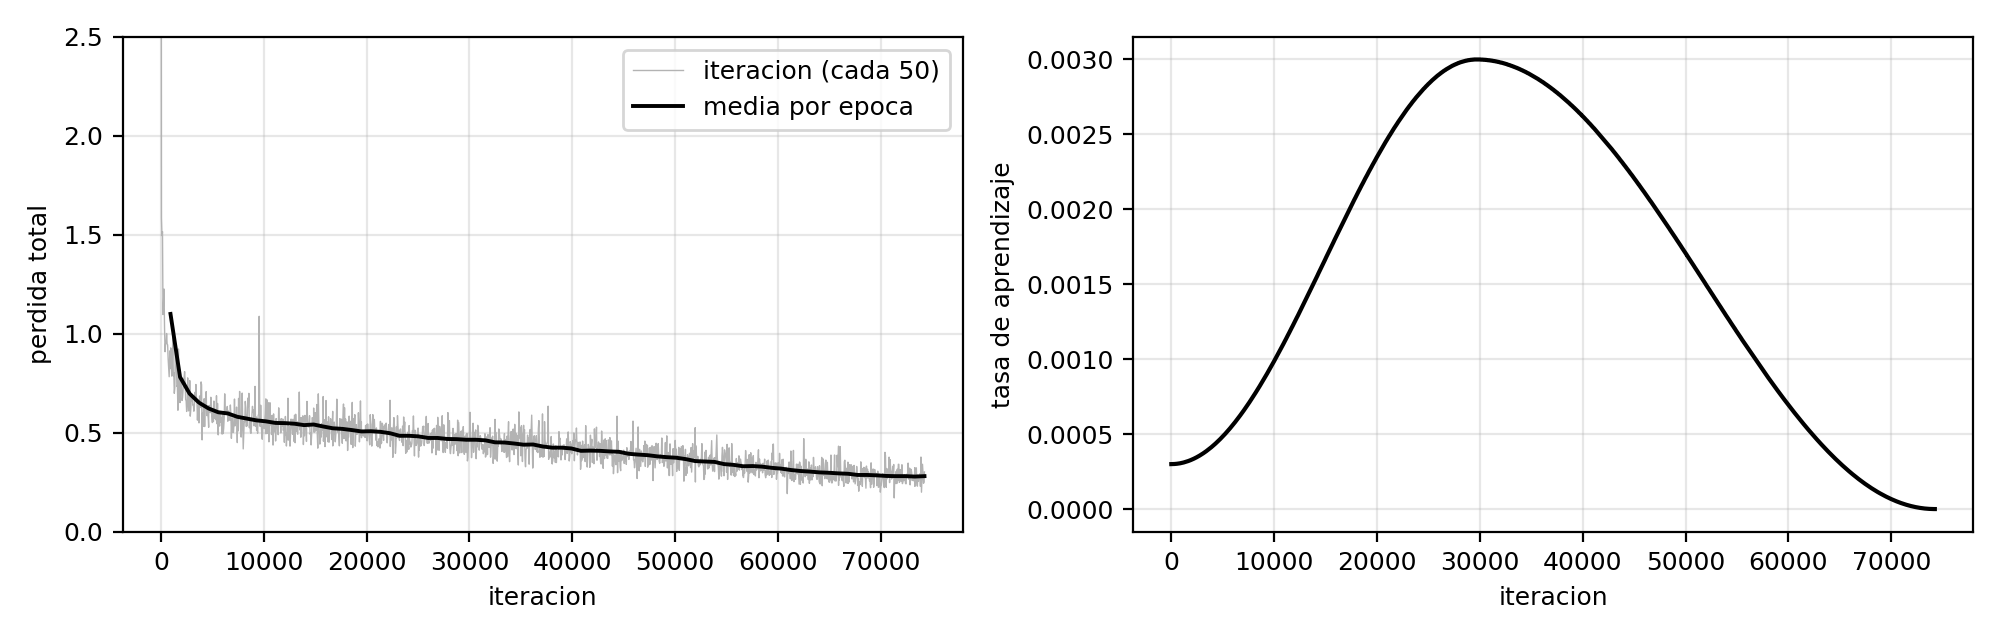
\includegraphics[width=0.85\textwidth]{curva_entrenamiento.png}
\caption{Entrenamiento propio de SECOND. Izquierda: pérdida total registrada cada 50 iteraciones (gris) y media por época (negro). Derecha: tasa de aprendizaje de la política de un ciclo.}
\label{fig:entrenamiento}
\end{figure}

\subsection{Desempeño en el conjunto de validación}

El modelo de la época 80 se evaluó sobre las 3\,769 escenas de validación con el código oficial de KITTI incluido en OpenPCDet. Con el mismo procedimiento se evaluaron los pesos preentrenados que publica OpenPCDet, obtenidos con la misma configuración. La Tabla \ref{tab:propios} presenta ambos resultados con 40 umbrales.

\begin{table}[htbp]
\caption{AP (\%) con 40 umbrales de SECOND en el conjunto de validación de KITTI. \textit{Propio}: modelo entrenado en este trabajo (época 80). \textit{Preentrenado}: pesos publicados por OpenPCDet \cite{openpcdet}, evaluados en este trabajo. NVIDIA GeForce RTX 5060, CUDA 12.8, PyTorch 2.7.1.}
\label{tab:propios}
\centering
\small
\begin{tabular}{@{}lllcccccc@{}}
\toprule
 & & & \multicolumn{3}{c}{\textbf{AP$_{3D}$}} & \multicolumn{3}{c}{\textbf{AP$_{\text{BEV}}$}} \\
\cmidrule(lr){4-6} \cmidrule(l){7-9}
\textbf{Clase} & \textbf{IoU} & \textbf{Pesos} & \textbf{Fácil} & \textbf{Mod.} & \textbf{Difícil} & \textbf{Fácil} & \textbf{Mod.} & \textbf{Difícil} \\
\midrule
Automóvil & 0,70 & Propio       & 89,50 & 81,09 & 78,21 & 91,93 & 88,21 & 87,27 \\
          &      & Preentrenado & 90,55 & 81,61 & 78,60 & 92,42 & 88,55 & 87,65 \\
\addlinespace[2pt]
Peatón    & 0,50 & Propio       & 55,79 & 51,23 & 46,90 & 60,52 & 56,16 & 52,22 \\
          &      & Preentrenado & 55,95 & 51,15 & 46,17 & 60,74 & 56,57 & 52,14 \\
\addlinespace[2pt]
Ciclista  & 0,50 & Propio       & 81,63 & 65,93 & 61,91 & 85,33 & 69,85 & 66,00 \\
          &      & Preentrenado & 82,96 & 66,73 & 62,78 & 88,05 & 71,16 & 66,89 \\
\bottomrule
\end{tabular}
\end{table}

En el nivel moderado, el modelo propio alcanza una AP$_{3D}$ de 81,09 en automóvil, 51,23 en peatón y 65,93 en ciclista. Las diferencias con los pesos preentrenados van de $-2{,}72$ a $+0{,}73$ puntos en las 18 cifras de la tabla; en AP$_{3D}$ moderado son de $-0{,}52$ en automóvil, $+0{,}08$ en peatón y $-0{,}80$ en ciclista. La mayor diferencia aparece en la AP$_{\text{BEV}}$ fácil de ciclista. La brecha entre clases se mantiene en el modelo propio: en el nivel moderado, el peatón queda 29,86 puntos por debajo del automóvil y el ciclista 15,16 puntos. El ciclista tiene la mayor caída entre los niveles fácil y difícil, 19,72 puntos de AP$_{3D}$, frente a 8,89 del peatón. La inferencia tomó 0,0283\,s por escena con ambos modelos.

Los pesos preentrenados ya se habían evaluado en el segundo avance del proyecto. Las cifras de la Tabla \ref{tab:propios} difieren de aquella evaluación en 0,02 puntos o menos, una variación atribuible al no determinismo de algunas operaciones en GPU y despreciable frente a las diferencias que se discuten.

\subsection{Comparación con la literatura}

El artículo original de SECOND \cite{yan2018} y la tabla de resultados de OpenPCDet reportan la AP con 11 umbrales, por lo que la comparación con ellos se hace con esa variante, que el código de evaluación también entrega. La Tabla \ref{tab:literatura} recoge la clase automóvil, la única que el artículo reporta en validación.

\begin{table}[htbp]
\caption{AP (\%) con 11 umbrales de SECOND en el conjunto de validación de KITTI, clase automóvil (IoU 0,70).}
\label{tab:literatura}
\centering
\small
\begin{tabular}{@{}lcccccc@{}}
\toprule
 & \multicolumn{3}{c}{\textbf{AP$_{3D}$}} & \multicolumn{3}{c}{\textbf{AP$_{\text{BEV}}$}} \\
\cmidrule(lr){2-4} \cmidrule(l){5-7}
\textbf{Fuente} & \textbf{Fácil} & \textbf{Mod.} & \textbf{Difícil} & \textbf{Fácil} & \textbf{Mod.} & \textbf{Difícil} \\
\midrule
Yan et al.\ \cite{yan2018}          & 87,43 & 76,48 & 69,10 & 89,96 & 87,07 & 79,66 \\
Preentrenado (evaluación propia)    & 88,61 & 78,62 & 77,20 & 90,01 & 87,91 & 86,46 \\
Propio                              & 87,77 & 78,19 & 76,95 & 89,75 & 87,57 & 85,99 \\
\midrule
Propio $-$ Yan et al.               & 0,34 & 1,71 & 7,85 & $-0{,}21$ & 0,50 & 6,33 \\
\bottomrule
\end{tabular}
\end{table}

El modelo propio supera al artículo original en AP$_{3D}$ en los tres niveles, con 1,71 puntos en el moderado y 7,85 en el difícil. En AP$_{\text{BEV}}$ la diferencia es pequeña en los niveles fácil y moderado y vuelve a ser amplia en el difícil (6,33 puntos). Para las tres clases, OpenPCDet publica la AP$_{3D}$ moderada de sus pesos: 78,62 en automóvil, 52,98 en peatón y 67,15 en ciclista \cite{openpcdet}. El modelo propio obtiene 78,19, 52,66 y 65,85, es decir, 0,43, 0,32 y 1,30 puntos menos. Los pesos preentrenados evaluados en este trabajo dan 78,62, 52,99 y 67,13, lo que confirma que el código de evaluación reproduce la cifra publicada. Como referencia adicional, sobre el conjunto de prueba oficial los autores de SECOND reportan una AP$_{3D}$ moderada de 73,66 en automóvil, 42,56 en peatón y 53,85 en ciclista \cite{yan2018}; esas cifras no son comparables con las de validación porque provienen de otro conjunto de escenas.

\subsection{Convergencia}

La Figura \ref{fig:convergencia} muestra la AP$_{3D}$ moderada en validación de los puntos de control de las épocas 20, 40, 60 y 80. En la época 20 el modelo ya obtiene 71,99 en automóvil, 39,48 en peatón y 59,22 en ciclista. Entre las épocas 20 y 40 el automóvil retrocede 3,50 puntos, mientras peatón y ciclista mejoran. Entre las épocas 40 y 60 el automóvil gana 10,10 puntos, y entre la 60 y la 80 el peatón gana 6,94, la mayor mejora de esa clase.

\begin{figure}[htbp]
\centering
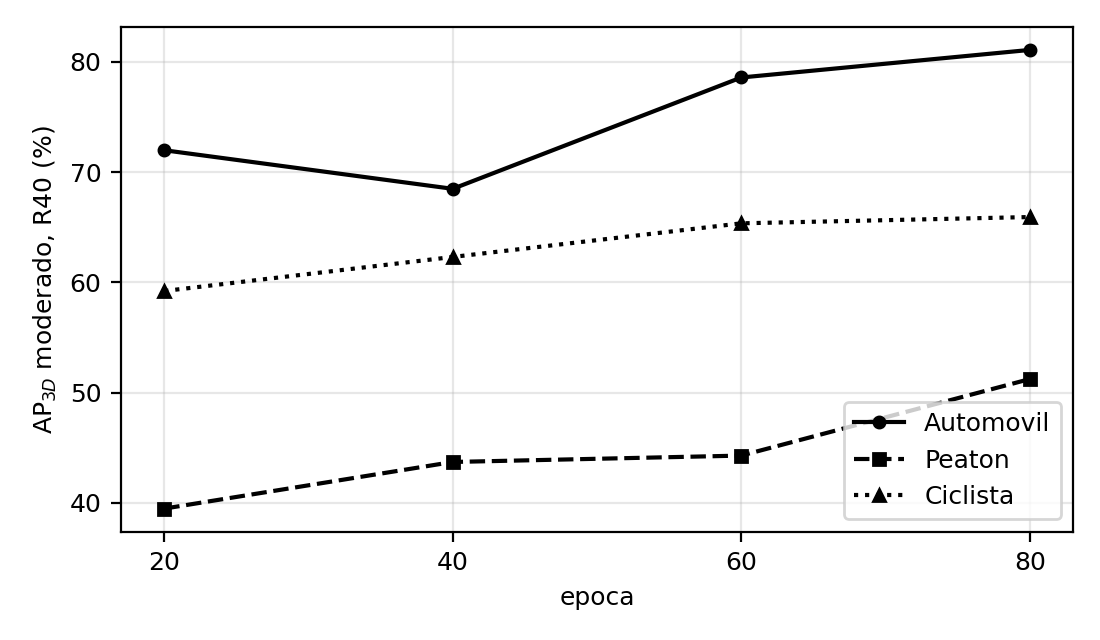
\includegraphics[width=0.5\textwidth]{ap_por_epoca.png}
\caption{AP$_{3D}$ moderada con 40 umbrales en el conjunto de validación, por época de entrenamiento.}
\label{fig:convergencia}
\end{figure}

\subsection{Exhaustividad por franja de distancia}

La Tabla \ref{tab:distancia} presenta la exhaustividad por clase y franja de distancia, calculada como se describe en el protocolo de evaluación, con puntaje mínimo de 0,3.

\begin{table}[htbp]
\caption{Exhaustividad (\%) por franja de distancia al sensor en el conjunto de validación (puntaje $\geq 0{,}3$; IoU 3D $\geq 0{,}7$ en automóvil y $\geq 0{,}5$ en peatón y ciclista). Entre paréntesis, objetos detectados sobre el total de la franja con el modelo propio.}
\label{tab:distancia}
\centering
\small
\begin{tabular}{@{}llrrr@{}}
\toprule
\textbf{Clase} & \textbf{Pesos} & \textbf{0--20\,m} & \textbf{20--40\,m} & \textbf{40--70,4\,m} \\
\midrule
Automóvil & Propio       & 93,98 (3\,559/3\,787) & 82,88 (4\,731/5\,708) & 55,59 (816/1\,468) \\
          & Preentrenado & 94,22 & 82,95 & 55,45 \\
\addlinespace[2pt]
Peatón    & Propio       & 70,22 (1\,080/1\,538) & 58,36 (328/562) & 12,50 (9/72) \\
          & Preentrenado & 68,66 & 54,80 & 18,06 \\
\addlinespace[2pt]
Ciclista  & Propio       & 84,19 (181/215) & 71,38 (207/290) & 61,05 (58/95) \\
          & Preentrenado & 83,72 & 74,14 & 60,00 \\
\bottomrule
\end{tabular}
\end{table}

La exhaustividad cae con la distancia en las tres clases. Entre la primera y la última franja, el modelo propio pierde 38,39 puntos en automóvil, 57,72 en peatón y 23,14 en ciclista. En la franja de 40 a 70,4\,m detecta solo 9 de los 72 peatones evaluables. Los dos modelos se comportan de forma muy parecida en automóvil; en peatón y ciclista las diferencias por franja llegan a algunos puntos, pero las franjas lejanas contienen pocos objetos y cada uno pesa más de un punto porcentual.

\subsection{Ejemplos cualitativos}

La Figura \ref{fig:cualitativo} muestra las predicciones del modelo propio sobre dos escenas de validación, las mismas que se analizaron con los pesos preentrenados en el segundo avance. En la escena 000201 (izquierda) hay 12 objetos anotados. El modelo detecta seis automóviles, entre 6,6 y 44,1\,m, y los dos ciclistas, con la clase correcta aunque están junto a un automóvil. Pierde un automóvil con oclusión fuerte a 40,3\,m, los dos peatones situados a 50,0\,m y un automóvil completamente truncado junto al vehículo de captura, que no entra en la evaluación. Produce tres falsos positivos de automóvil: a 24,0\,m con puntaje 0,605, a 34,4\,m con 0,362 y a 60,2\,m con 0,309. El primero también aparecía con los pesos preentrenados, con puntaje 0,504. En la escena 000124 (derecha) todos los objetos están a más de 40\,m. El modelo solo detecta el automóvil a 53,2\,m, con puntaje 0,466, y pierde un automóvil ocluido a 41,3\,m, un ciclista a 58,2\,m y dos peatones a 58,7 y 59,3\,m. Añade dos falsos positivos con puntaje bajo: un automóvil a 43,9\,m (0,379) y un ciclista a 45,7\,m (0,344).

\begin{figure}[htbp]
\centering
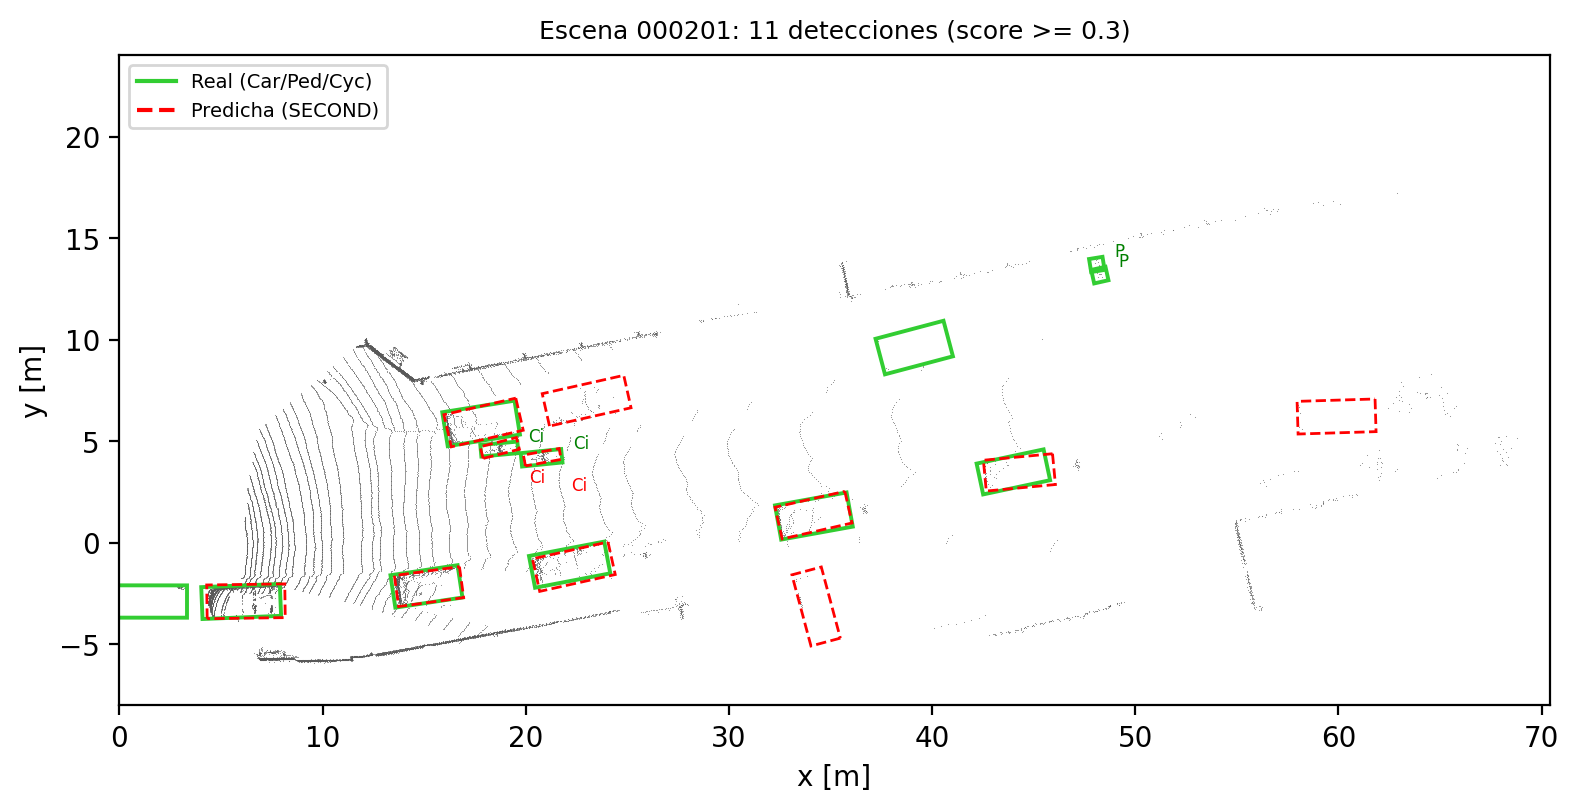
\includegraphics[height=5.2cm]{pred_propio_000201.png}\hfill
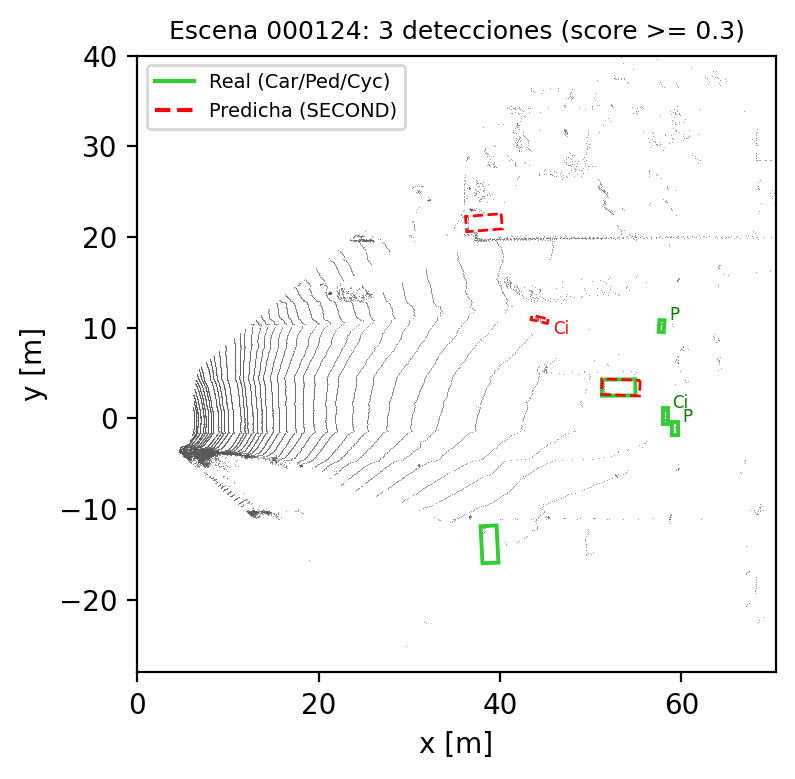
\includegraphics[height=5.2cm]{pred_propio_000124.png}
\caption{Predicciones del modelo propio en vista de pájaro sobre dos escenas del conjunto de validación de KITTI: 000201 (izquierda) y 000124 (derecha). Verde continuo: anotación real de automóvil, peatón o ciclista; rojo discontinuo: predicción con puntaje mayor o igual a 0,3. Las letras P y Ci marcan peatones y ciclistas. Solo se dibujan los puntos dentro del campo de visión de la cámara, que son los que recibe el modelo.}
\label{fig:cualitativo}
\end{figure}

% ================================================================= Discusión
\section{Discusión}
\label{sec:discusion}

\textbf{Reproducción del desempeño publicado.} El entrenamiento propio alcanzó prácticamente el mismo desempeño que los pesos de referencia: 17 de las 18 cifras de la Tabla \ref{tab:propios} quedan a menos de 1,5 puntos, y con 11 umbrales el modelo queda a 0,43 puntos de la cifra publicada por OpenPCDet en automóvil moderado. Esto indica que la configuración descrita en la sección \ref{sec:metodologia} basta para reproducir el resultado. Las diferencias tienden a ser negativas, sobre todo en ciclista, pero no puede afirmarse que sean significativas: se hizo un solo entrenamiento y no se midió la variación entre corridas con distintas semillas, que en clases con pocos ejemplos, como el nivel difícil de ciclista con 96 objetos de entrenamiento, puede ser del mismo orden. Frente al artículo original, la mejora de 7,85 puntos en el nivel difícil de automóvil es la más notable. Como la arquitectura es la misma, la ganancia debe atribuirse a los ajustes de entrenamiento que incorporó la implementación de referencia; este trabajo no permite aislar cuál de ellos es responsable.

\textbf{Brecha entre clases.} La diferencia de casi 30 puntos entre automóvil y peatón se explica por los datos antes que por el modelo. El peatón tiene la menor AP$_{\text{BEV}}$, de modo que su dificultad empieza por localizarlo en el plano y no solo por estimar su altura. La Tabla \ref{tab:puntos} muestra por qué: más allá de 40\,m un peatón queda con una mediana de 11 puntos, una forma poco distinguible de un poste o de un arbusto, y en esa franja hay pocos ejemplos de entrenamiento. La exhaustividad de 12,50\% en la franja lejana (Tabla \ref{tab:distancia}) es la consecuencia directa. El ciclista, con una cantidad de puntos parecida a esa distancia (16), conserva una exhaustividad de 61,05\%; una explicación plausible es que su silueta, más larga, es más fácil de separar del fondo, pero los 95 ciclistas lejanos de validación no permiten confirmarlo. En automóvil, en cambio, la distancia entre AP$_{\text{BEV}}$ y AP$_{3D}$ es la mayor de las tres clases (7,12 puntos en el nivel moderado), lo que indica que buena parte de su error está en la altura y en la exigencia del umbral de IoU de 0,7.

\textbf{Convergencia.} El retroceso del automóvil entre las épocas 20 y 40 coincide con la fase de tasa de aprendizaje más alta, cuyo máximo se alcanza en la época 32 (el 40\% del entrenamiento). Las mayores ganancias llegan cuando la tasa desciende, lo que es coherente con el propósito de la política de un ciclo \cite{smith2017}. La mejora de 6,94 puntos del peatón en las últimas 20 épocas sugiere que esa clase aún no estaba saturada, aunque prolongar el entrenamiento no garantiza que la ganancia continúe.

\textbf{Modos de falla.} Los ejemplos cualitativos confirman lo que muestran las métricas. Los objetos que se pierden son lejanos, ocluidos o pequeños, y los falsos positivos son en su mayoría automóviles, con puntajes entre 0,309 y 0,605. El falso positivo a 24\,m de la escena 000201 aparece con los dos modelos, lo que sugiere que se debe a la geometría de la escena y no a una particularidad del entrenamiento. El modelo propio genera en la escena 000124 dos falsos positivos que el preentrenado no producía, ambos con puntaje inferior a 0,4. Con un umbral de 0,4 desaparecerían en estas dos escenas, aunque en el conjunto completo subir el umbral también reduce la exhaustividad.

\textbf{Relación con el estado del arte.} Las debilidades observadas coinciden con las que atacan los trabajos recientes de la Tabla \ref{tab:comparativa}. EAS-Det \cite{wang2025eas} reporta sus mayores ganancias precisamente en peatón y ciclista, Zhao et al.\ \cite{zhao2025} adaptan el procesamiento a la densidad de puntos y FGVoxel3D \cite{ao2026} cuestiona la resolución única de vóxel, que con 0,05\,m deja a un peatón lejano, con una mediana de 11 puntos, representado por muy pocos vóxeles ocupados. Los resultados de este trabajo cuantifican el margen sobre el que operan esas propuestas: en la línea base reproducida, el problema no es el automóvil cercano, que se detecta en el 93,98\% de los casos, sino el peatón a más de 40\,m.

\textbf{Limitaciones.} Las cifras provienen de un único entrenamiento. Se reportan sobre el conjunto de validación, porque las etiquetas de prueba de KITTI no son públicas. KITTI no incluye escenas nocturnas ni de clima adverso \cite{dong2023}. Además, la exhaustividad por distancia depende del umbral de puntaje elegido y no considera los falsos positivos, por lo que complementa a la AP pero no la sustituye.

% ============================================================= Conclusiones
\section{Conclusiones y trabajo futuro}
\label{sec:conclusiones}

Se entrenó desde cero el detector SECOND sobre KITTI con la configuración de la implementación de referencia, en una sola tarjeta gráfica de consumo y en 6\,h 28\,min 52\,s. El modelo obtuvo en el conjunto de validación una AP$_{3D}$ moderada, con 40 umbrales, de 81,09 en automóvil, 51,23 en peatón y 65,93 en ciclista. Estas cifras quedan a menos de un punto de las que obtienen, en las mismas condiciones, los pesos publicados por OpenPCDet, y superan las del artículo original en automóvil, de modo que el objetivo de reproducir el desempeño publicado se cumplió.

El análisis mostró que el desempeño depende sobre todo de la distancia y de la clase. La exhaustividad de automóvil pasa de 93,98\% en los primeros 20\,m a 55,59\% más allá de 40\,m, y la de peatón cae a 12,50\% en esa franja, en correspondencia con la pérdida de puntos LiDAR que cuantificó el análisis exploratorio. La brecha de casi 30 puntos entre automóvil y peatón se explica por la escasez de puntos y de ejemplos, más que por un defecto del entrenamiento.

Como trabajo futuro se propone, en primer lugar, repetir el entrenamiento con varias semillas para estimar la variación entre corridas y saber qué diferencias son significativas. En segundo lugar, evaluar sobre esta misma línea base uno de los módulos de mejora de la Tabla \ref{tab:comparativa} orientados a objetos lejanos y clases minoritarias, o el refinamiento sobre atributos de vóxel de Voxel R-CNN \cite{deng2021}, usando la exhaustividad por distancia como métrica de seguimiento. Por último, medir la robustez del modelo ante corrupciones de la nube de puntos \cite{dong2023, li2026}, que KITTI no permite evaluar de forma directa.

% ============================================================== Referencias
\begin{thebibliography}{99}
\footnotesize
\setlength{\itemsep}{0pt}

\bibitem{geiger2013}
A. Geiger, P. Lenz, C. Stiller y R. Urtasun, ``Vision meets robotics: The KITTI dataset,'' \emph{The International Journal of Robotics Research}, vol. 32, n.\textordmasculine{} 11, pp. 1231--1237, 2013.

\bibitem{qian2022}
R. Qian, X. Lai y X. Li, ``3D object detection for autonomous driving: A survey,'' \emph{Pattern Recognition}, vol. 130, art. 108796, 2022.

\bibitem{zamanakos2021}
G. Zamanakos, L. Tsochatzidis, A. Amanatiadis e I. Pratikakis, ``A comprehensive survey of LIDAR-based 3D object detection methods with deep learning for autonomous driving,'' \emph{Computers \& Graphics}, vol. 99, pp. 153--181, 2021.

\bibitem{cai2025}
J. Cai y Y. Wu, ``Three-dimensional object detection for autonomous driving via deep learning: A review,'' \emph{Engineering Applications of Artificial Intelligence}, 2025, doi: 10.1016/j.engappai.2025.112238.

\bibitem{shi2025}
Y. Shi, B. Guo, L. Jin, X. Yang, H. Zhang, X. Liu y M. Li, ``Towards cognition-driven 3D object detection: A LiDAR-based framework,'' \emph{Knowledge-Based Systems}, 2025, doi: 10.1016/j.knosys.2025.115051.

\bibitem{sohail2025}
S. S. Sohail, Y. Himeur, H. Kheddar, A. Amira, F. Fadli, S. Atalla, A. Copiaco y W. Mansoor, ``Advancing 3D point cloud understanding through deep transfer learning: A comprehensive survey,'' \emph{Information Fusion}, vol. 113, art. 102601, 2025, doi: 10.1016/j.inffus.2024.102601.

\bibitem{guo2021}
Y. Guo, H. Wang, Q. Hu, H. Liu, L. Liu y M. Bennamoun, ``Deep learning for 3D point clouds: A survey,'' \emph{IEEE Transactions on Pattern Analysis and Machine Intelligence}, vol. 43, n.\textordmasculine{} 12, pp. 4338--4364, 2021.

\bibitem{li2021}
Y. Li, L. Ma, Z. Zhong, F. Liu, M. A. Chapman, D. Cao y J. Li, ``Deep learning for LiDAR point clouds in autonomous driving: A review,'' \emph{IEEE Transactions on Neural Networks and Learning Systems}, vol. 32, n.\textordmasculine{} 8, pp. 3412--3432, 2021.

\bibitem{shi2021}
S. Shi, Z. Wang, J. Shi, X. Wang y H. Li, ``From points to parts: 3D object detection from point cloud with part-aware and part-aggregation network,'' \emph{IEEE Transactions on Pattern Analysis and Machine Intelligence}, vol. 43, n.\textordmasculine{} 8, pp. 2647--2664, 2021.

\bibitem{yan2018}
Y. Yan, Y. Mao y B. Li, ``SECOND: Sparsely embedded convolutional detection,'' \emph{Sensors}, vol. 18, n.\textordmasculine{} 10, art. 3337, 2018.

\bibitem{erabati2024a}
G. K. Erabati y H. Araujo, ``SRFDet3D: Sparse region fusion based 3D object detection,'' \emph{Neurocomputing}, vol. 593, art. 127814, 2024, doi: 10.1016/j.neucom.2024.127814.

\bibitem{erabati2024b}
G. K. Erabati y H. Araujo, ``DeLiVoTr: Deep and light-weight voxel transformer for 3D object detection,'' \emph{Intelligent Systems with Applications}, vol. 22, art. 200361, 2024.

\bibitem{qi2024}
Y. Qi, C. Liu, M. Scaioni, Y. Li, Y. Qiao, X. Ma, H. Wu, K. Zhang y D. Wang, ``Geometric information constraint 3D object detection from LiDAR point cloud for autonomous vehicles under adverse weather,'' \emph{Transportation Research Part C: Emerging Technologies}, vol. 161, art. 104555, 2024, doi: 10.1016/j.trc.2024.104555.

\bibitem{an2026}
Y. An y F. Li, ``LiDAR point clouds segmentation in adverse weather conditions,'' \emph{Signal Processing}, vol. 239, art. 110256, 2026, doi: 10.1016/j.sigpro.2025.110256.

\bibitem{liu2025}
Y. Liu, Y. Zhang, R. Lan, C. Cheng y Z. Wu, ``AWARDistill: Adaptive and robust 3D object detection in adverse conditions through knowledge distillation,'' \emph{Expert Systems with Applications}, vol. 266, art. 126032, 2025.

\bibitem{pravallika2024}
A. Pravallika, M. F. Hashmi y A. Gupta, ``Deep learning frontiers in 3D object detection: A comprehensive review for autonomous driving,'' \emph{IEEE Access}, vol. 12, pp. 173936--173980, 2024.

\bibitem{liu2023}
H. Liu, C. Wu y H. Wang, ``Real time object detection using LiDAR and camera fusion for autonomous driving,'' \emph{Scientific Reports}, vol. 13, 2023.

\bibitem{caesar2020}
H. Caesar, V. Bankiti, A. H. Lang, S. Vora, V. E. Liong, Q. Xu, A. Krishnan, Y. Pan, G. Baldan y O. Beijbom, ``nuScenes: A multimodal dataset for autonomous driving,'' en \emph{Proc. IEEE/CVF Conference on Computer Vision and Pattern Recognition (CVPR)}, 2020, pp. 11621--11631.

\bibitem{yang2018}
B. Yang, W. Luo y R. Urtasun, ``PIXOR: Real-time 3D object detection from point clouds,'' en \emph{Proc. IEEE/CVF Conference on Computer Vision and Pattern Recognition (CVPR)}, 2018, pp. 7652--7660.

\bibitem{zhou2018}
Y. Zhou y O. Tuzel, ``VoxelNet: End-to-end learning for point cloud based 3D object detection,'' en \emph{Proc. IEEE/CVF Conference on Computer Vision and Pattern Recognition (CVPR)}, 2018, pp. 4490--4499.

\bibitem{lang2019}
A. H. Lang, S. Vora, H. Caesar, L. Zhou, J. Yang y O. Beijbom, ``PointPillars: Fast encoders for object detection from point clouds,'' en \emph{Proc. IEEE/CVF Conference on Computer Vision and Pattern Recognition (CVPR)}, 2019, pp. 12697--12705.

\bibitem{shi2019}
S. Shi, X. Wang y H. Li, ``PointRCNN: 3D object proposal generation and detection from point cloud,'' en \emph{Proc. IEEE/CVF Conference on Computer Vision and Pattern Recognition (CVPR)}, 2019, pp. 770--779.

\bibitem{shi2020}
S. Shi, C. Guo, L. Jiang, Z. Wang, J. Shi, X. Wang y H. Li, ``PV-RCNN: Point-voxel feature set abstraction for 3D object detection,'' en \emph{Proc. IEEE/CVF Conference on Computer Vision and Pattern Recognition (CVPR)}, 2020.

\bibitem{deng2021}
J. Deng, S. Shi, P. Li, W. Zhang, H. Zhang y H. Li, ``Voxel R-CNN: Towards high performance voxel-based 3D object detection,'' en \emph{Proc. AAAI Conference on Artificial Intelligence}, vol. 35, 2021, pp. 1201--1209.

\bibitem{yin2021}
T. Yin, X. Zhou y P. Krähenbühl, ``Center-based 3D object detection and tracking,'' en \emph{Proc. IEEE/CVF Conference on Computer Vision and Pattern Recognition (CVPR)}, 2021, pp. 11784--11793.

\bibitem{chen2022b}
Y. Chen, Y. Li, X. Zhang, J. Sun y J. Jia, ``Focal sparse convolutional networks for 3D object detection,'' en \emph{Proc. IEEE/CVF Conference on Computer Vision and Pattern Recognition (CVPR)}, 2022, pp. 5428--5437.

\bibitem{dong2023}
Y. Dong, C. Kang, J. Zhang, Z. Zhu, Y. Wang, X. Yang, H. Su, X. Wei y J. Zhu, ``Benchmarking robustness of 3D object detection to common corruptions,'' en \emph{Proc. IEEE/CVF Conference on Computer Vision and Pattern Recognition (CVPR)}, 2023, pp. 1022--1032.

\bibitem{ke2025}
Z. Ke, C. Lin, T. Zhang, T. Jia, M. Du, G. Wang y Y. Zhang, ``Multi-feature enhancement based on sparse networks for single-stage 3D object detection,'' \emph{Alexandria Engineering Journal}, vol. 111, pp. 123--135, 2025.

\bibitem{ao2026}
L. Ao, X. Wang, W. Wan, N. Ouyang, Q. Li y K. Sheng, ``FGVoxel3D: Fine-grained multi-resolution voxel network for 3D object detection,'' \emph{Neurocomputing}, vol. 659, art. 131702, 2026, doi: 10.1016/j.neucom.2025.131702.

\bibitem{wang2025iavt}
B. Wang, C. Xia, X. Gao, Y. Yang, K.-C. Li, X. Fang, Y. Zhang y S. Ge, ``Instance-aware sampling and voxel-transformer encoding for single-stage 3D object detection,'' \emph{Digital Signal Processing}, vol. 162, art. 105171, 2025, doi: 10.1016/j.dsp.2025.105171.

\bibitem{chen2025sp}
T. Chen, Y. Yuan, B. Yin y Y. Liao, ``SP-Pillars: An efficient LiDAR 3D objects detection framework with multi-scale feature perception and optimization,'' \emph{IEEE Access}, vol. 13, pp. 74092--74106, 2025, doi: 10.1109/ACCESS.2025.3564665.

\bibitem{xu2025}
H. Xu, L. Yang, S. Zhao, S. Tao, X. Tian y K. Liu, ``SPS-RCNN: Semantic-guided proposal sampling for 3D object detection from LiDAR point clouds,'' \emph{Sensors}, vol. 25, n.\textordmasculine{} 4, art. 1064, 2025, doi: 10.3390/s25041064.

\bibitem{yin2026}
X. Yin, Z. Xiao, J. Shao, Z. Qiu y L. Wang, ``HFSA-Net: A 3D object detection network with structural encoding and attention enhancement for LiDAR point clouds,'' \emph{Sensors}, vol. 26, n.\textordmasculine{} 1, art. 338, 2026, doi: 10.3390/s26010338.

\bibitem{zhao2025}
J. Zhao, J. Li, W. Zhou, H. Ren, Y. Long y H. Hu, ``Density-aware tree--graph cross-message passing for LiDAR point cloud 3D object detection,'' \emph{Remote Sensing}, vol. 17, n.\textordmasculine{} 13, art. 2177, 2025, doi: 10.3390/rs17132177.

\bibitem{wang2025eas}
H. Wang, J. Ma, Y. Zhao, J. Zhang y F. Chen, ``EAS-Det: Edge-aware semantic feature fusion for robust 3D object detection in LiDAR point clouds,'' \emph{Remote Sensing}, vol. 17, n.\textordmasculine{} 22, art. 3743, 2025, doi: 10.3390/rs17223743.

\bibitem{li2026}
X. Li, X. Sun, J. Li, Y. Ji y W. Fu, ``Bounded graph conditioning for LiDAR 3D object detection under sensor degradation,'' \emph{Sensors}, vol. 26, n.\textordmasculine{} 9, art. 2667, 2026, doi: 10.3390/s26092667.

\bibitem{ju2026}
X. Ju, R. Zhou, F. Fang, S. Li, Y. Xiao, J. Liu y Z. Xu, ``LiDAR adverse-weather simulation with ground effect for robust 3D object detection,'' \emph{Applied Sciences}, vol. 16, n.\textordmasculine{} 9, art. 4409, 2026, doi: 10.3390/app16094409.

\bibitem{wirges2018}
S. Wirges, T. Fischer, C. Stiller y J. B. Frias, ``Object detection and classification in occupancy grid maps using deep convolutional networks,'' en \emph{Proc. IEEE International Conference on Intelligent Transportation Systems (ITSC)}, 2018.

\bibitem{chen2015}
X. Chen, K. Kundu, Y. Zhu, A. G. Berneshawi, H. Ma, S. Fidler y R. Urtasun, ``3D object proposals for accurate object class detection,'' en \emph{Advances in Neural Information Processing Systems (NeurIPS)}, 2015.

\bibitem{lin2017}
T.-Y. Lin, P. Goyal, R. Girshick, K. He y P. Dollár, ``Focal loss for dense object detection,'' en \emph{Proc. IEEE International Conference on Computer Vision (ICCV)}, 2017, pp. 2980--2988.

\bibitem{smith2017}
L. N. Smith, ``Cyclical learning rates for training neural networks,'' en \emph{Proc. IEEE Winter Conference on Applications of Computer Vision (WACV)}, 2017, pp. 464--472.

\bibitem{simonelli2019}
A. Simonelli, S. R. Bulò, L. Porzi, M. López-Antequera y P. Kontschieder, ``Disentangling monocular 3D object detection,'' en \emph{Proc. IEEE/CVF International Conference on Computer Vision (ICCV)}, 2019, pp. 1991--1999.

\bibitem{openpcdet}
OpenPCDet Development Team, ``OpenPCDet: An open-source toolbox for 3D object detection from point clouds,'' 2020. [En línea]. Disponible en: \url{https://github.com/open-mmlab/OpenPCDet}

\end{thebibliography}

\end{document}
